\documentclass{beamer}
\usepackage{../../typesetting/styles/slide-zh}

% Document information
\title{\LARGE{周报}}
\subtitle{}
\author{}
\date{2025-04-07}

\begin{document}

% Title frame
\begin{frame}
  \titlepage
\end{frame}

% Outline frame
\begin{frame}{大纲}
  \tableofcontents
\end{frame}

% Paper Experiment
\section{论文实验}
\begin{frame}{实验数据收集}
  目前还差一个小章节的实验未做完
  \begin{block}{扩展更多参数集}
    \begin{itemize}
      \item 从SPHINCS$^+$-128F扩展到SPHINCS$^+$-128S和SPHINCS$^+$-192F
      \item 收集和分析运行时数据
      \item 完成性能评估与验证
    \end{itemize}
  \end{block}

  \begin{center}
    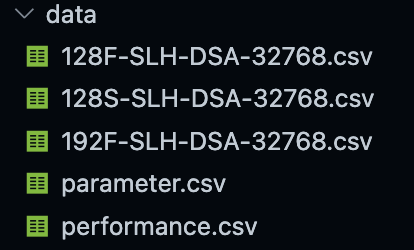
\includegraphics[width=0.5\textwidth]{./fig/data-collection.png}
  \end{center}
\end{frame}

\section{实验章节}

\begin{frame}{线程模型与性能分析}
  \begin{block}{线程模型参数与优化分配}
    通过实验建立的模型参数反映了不同操作在各参数集的计算特性:
    \begin{itemize}
      \item $\alpha_i$、$\beta_i$和$\gamma_i$ - 反映计算密度与特性
      \item $t_i^*$ - 根据模型计算出的最优线程数
      \item 不同安全级别和参数配置需要不同的线程分配策略以达到最佳性能
    \end{itemize}
  \end{block}

  \begin{center}
    \footnotesize
    \begin{tabular}{lrrrr}
      \toprule
      \textbf{操作} & \boldmath$\alpha_i$ & \boldmath$\beta_i$ & \boldmath$\gamma_i$ & \boldmath$t_i^*$ \\
      \midrule
      128F-密钥 & 52.06 & 506,000 & 1.26E-4 & 63,310 \\
      128F-签名 & 1,386 & 13,231,567 & 3.60E-3 & 60,636 \\
      128F-验证 & 164.72 & 1,395,012 & 4.54E-4 & 55,407 \\
      128S-密钥 & 3,317 & 32,046,199 & 7.15E-3 & 66,929 \\
      128S-签名 & 23,716 & 248,632,501 & 6.59E-2 & 61,419 \\
      128S-验证 & 63.22 & 484,914 & 1.44E-4 & 57,968 \\
      \bottomrule
    \end{tabular}
  \end{center}
\end{frame}

\begin{frame}{SLH-DSA实现性能比较}
  \begin{block}{性能提升亮点}
    \begin{itemize}
      \item 相比于基准实现,我们的方法在同样硬件下取得性能提升
      \item 通过自适应线程分配策略优化了GPU资源利用率
    \end{itemize}
  \end{block}
  \begin{center}
    \scriptsize
    \begin{tabular}{lccc}
      \toprule
      \textbf{实现} & \multicolumn{3}{c}{\textbf{吞吐量(任务/秒)}} \\
      \cmidrule(lr){2-4}
      & \textbf{公钥生成} & \textbf{签名} & \textbf{验证} \\
      \midrule
      128f \cite{Kim2024} & 725,118 (55\%) & 44,391 (97\%) & 285,681 (81\%) \\
      128f \cite{Wang2025} & 1,309,136 (100\%) & 45,425 (100\%) & 352,333 (100\%) \\
      128f \cite{Wang2025}$^\dagger$ & 1,435,690 (109.7\%) & 53,804 (118.4\%) & 451,883 (128.3\%) \\
      128f 本工作 & \textbf{1,587,849 (121.3\%)} & \textbf{62,239 (137.0\%)} & \textbf{502,243 (142.5\%)} \\
      \bottomrule
    \end{tabular}
  \end{center}

\end{frame}

\begin{frame}{老师评语}
  \begin{alertblock}{那个第1篇参考文献1994年的换成最近的,比如综述论文引用过这篇的,不要用20年前的参考文献}
    已替换为20年后文献
  \end{alertblock}
  \begin{alertblock}{加快推进可投稿}
    抓紧时间
  \end{alertblock}

  \begin{block}{下周计划}
    \begin{itemize}
      \item 完成最后一小章节FLP实验
      \item 对文章图片和段落进行润色
    \end{itemize}
  \end{block}
\end{frame}

% References
\begin{frame}
  \frametitle{参考文献}
  \bibliographystyle{alpha}
  \bibliography{../../paper}
\end{frame}

\end{document}
